
\begin{figure}[t]
    \centering
    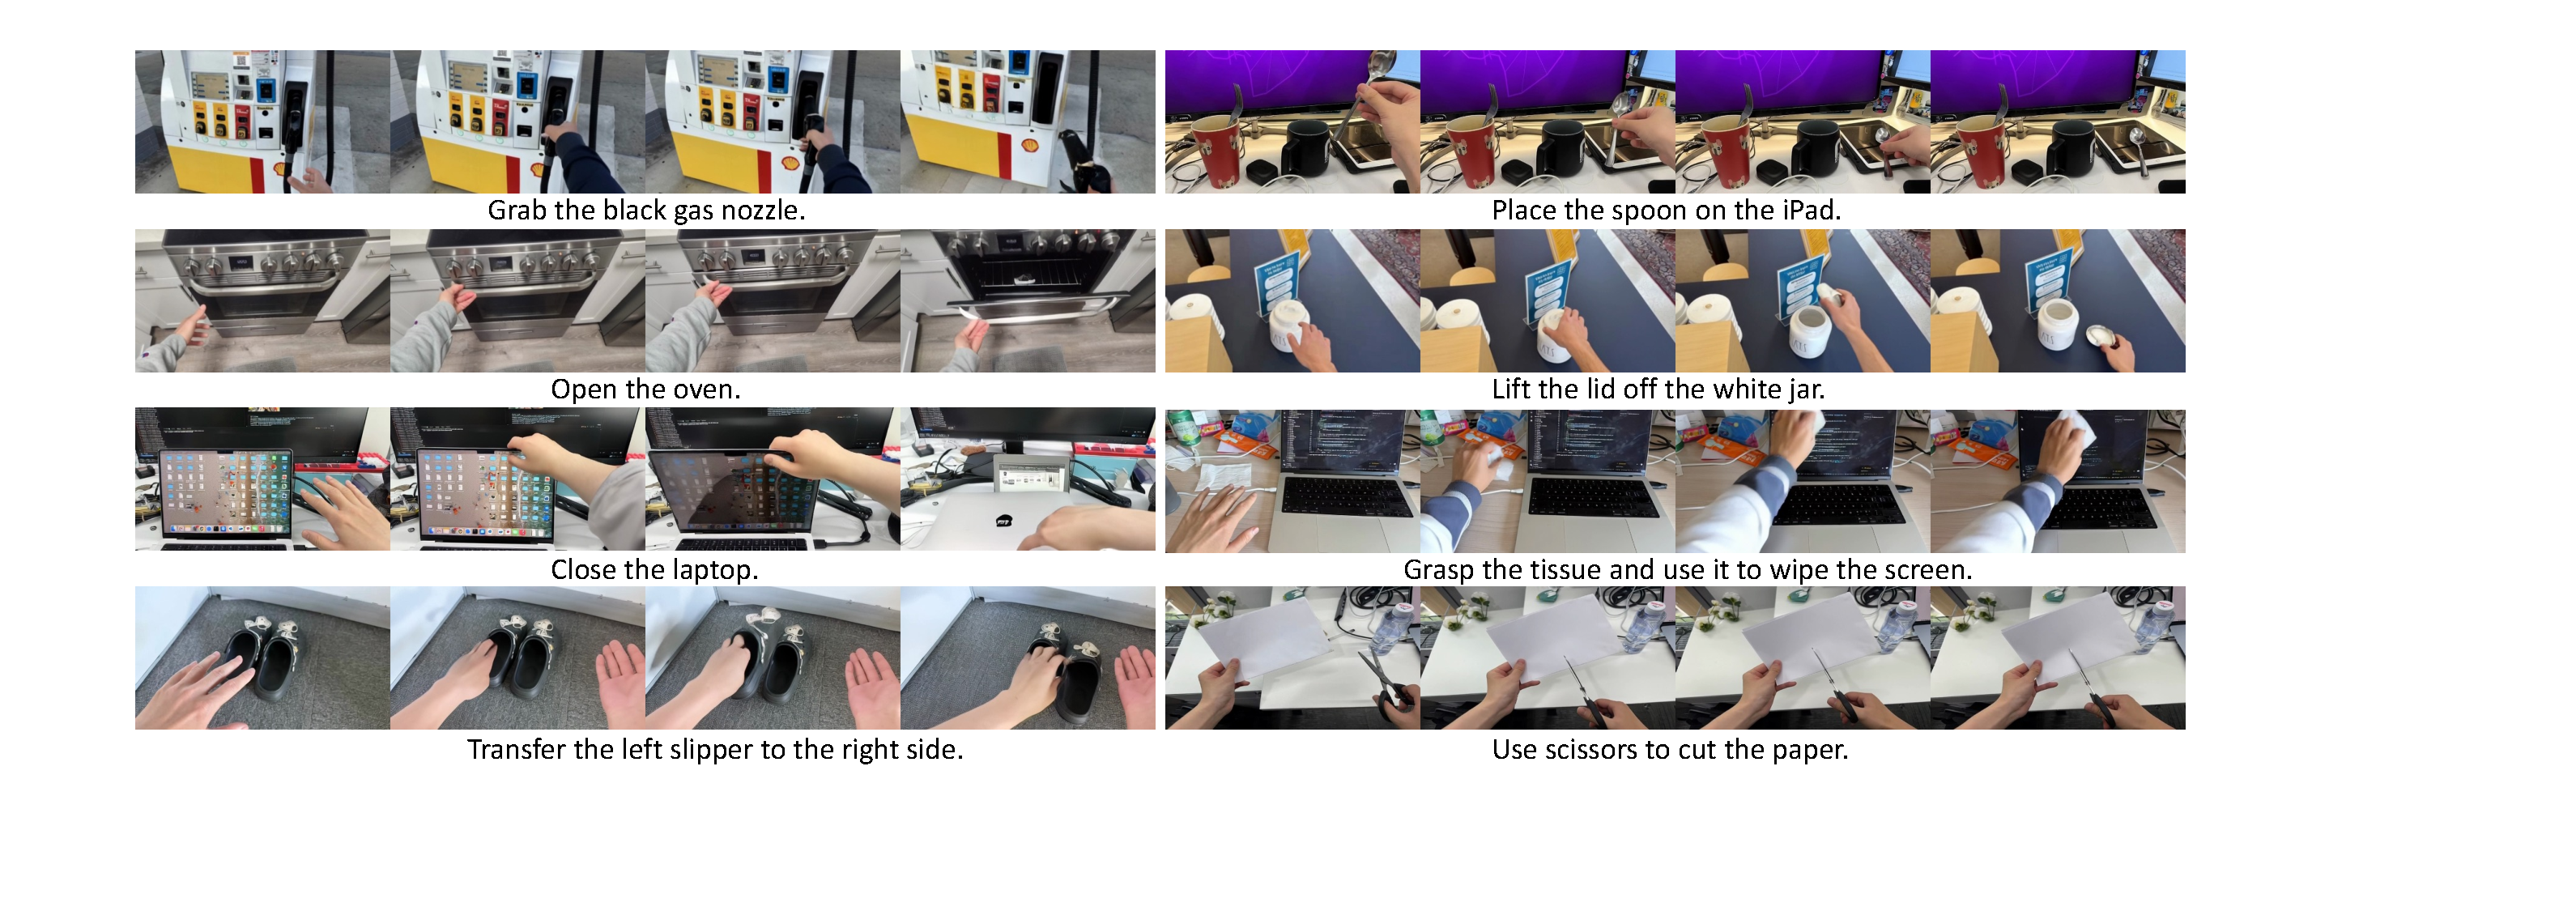
\includegraphics[width=1.0\linewidth]{figures/fig6.pdf}
    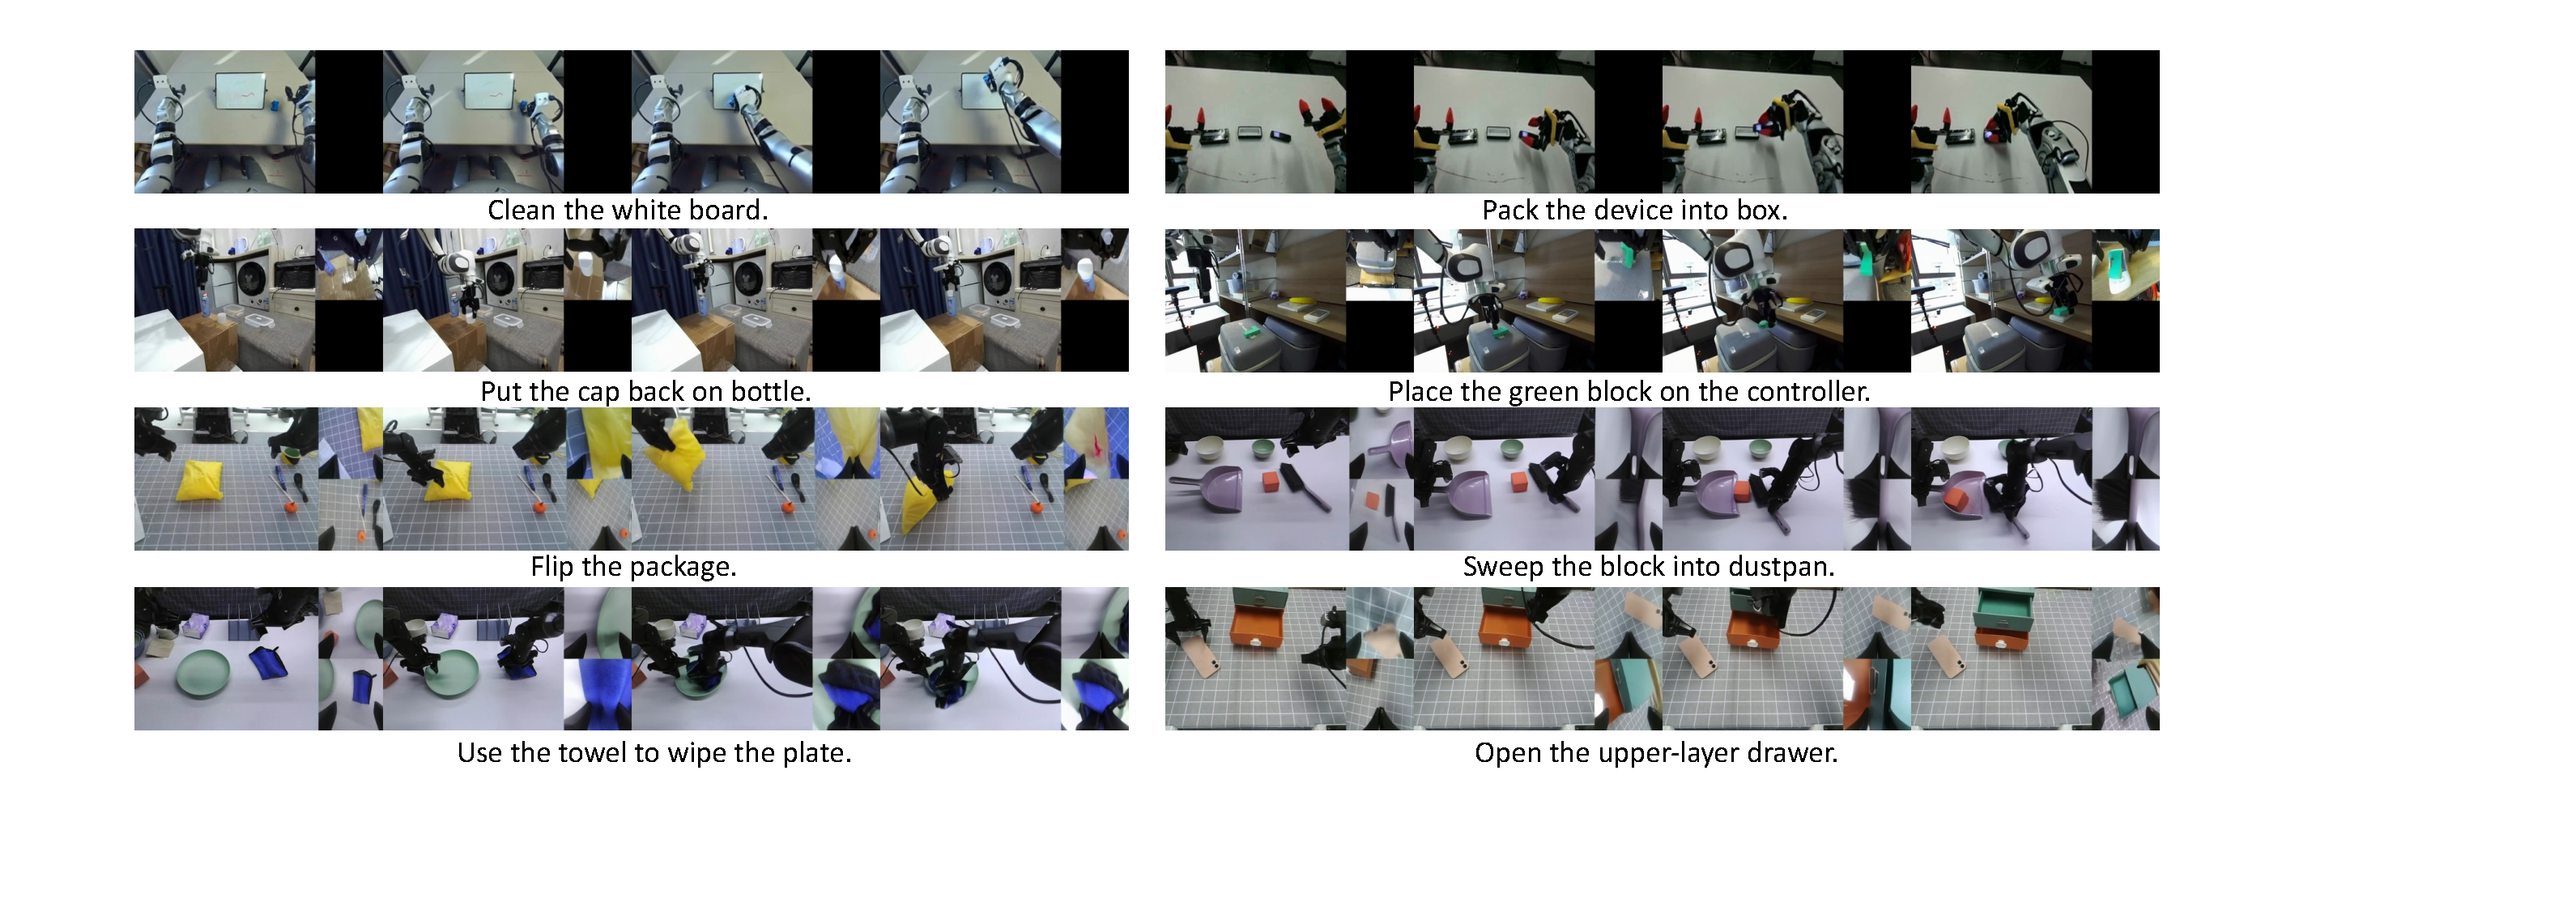
\includegraphics[width=1.0\linewidth]{figures/fig7.pdf}
    \caption{VPP2 video predictions for human-hand and robot manipulation. Trained on large-scale, diverse manipulation datasets, VPP2 generalizes across human hands and a wide range of robot embodiments. For robot manipulation, VPP2 jointly predicts one to three camera views arranged in a T-shaped composite. Due to space constraints, single-step video predictions after distillation are shown in Figure~\ref{fig:video_app} in the appendix.}
    \vspace{-4mm}
    \label{fig:fig6}
\end{figure}

% \begin{figure}[t]
%     \centering
%     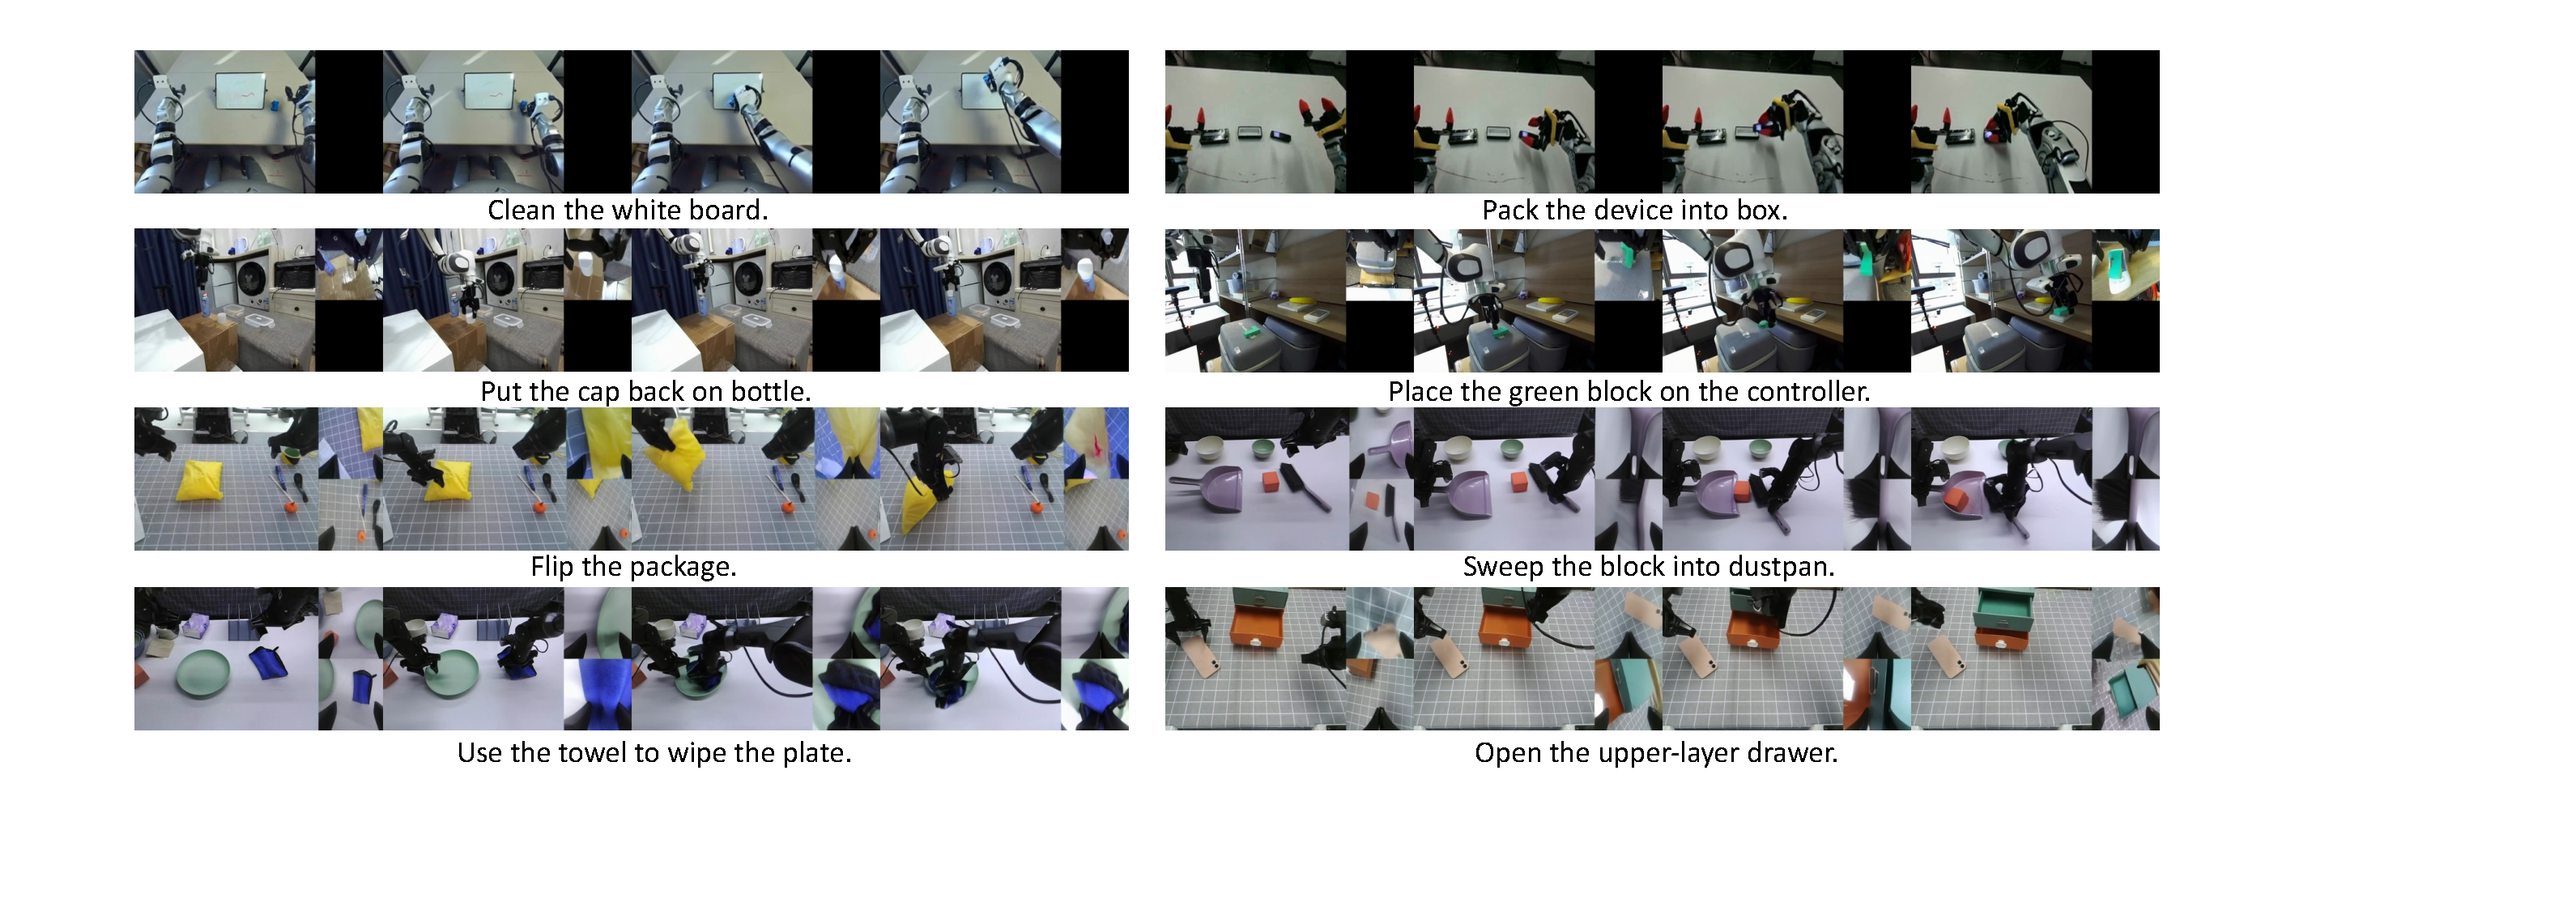
\includegraphics[width=1.0\linewidth]{figures/fig7.pdf}
%     \caption{VPP2 video predictions on robot manipulation video prediction. By training on large diverse robot datasets, VPP2 support different robot embodiment and different number of camera views (main-view is put in the left and two possible auxiliary views is put on the right side).}
%     \label{fig:fig7}
% \end{figure}

\section{Experiments}
In this section, we conduct experiments to answer the following questions:
(1) How does the motion quality of VPP2's video predictions compare with that of state-of-the-art video foundation models on manipulation tasks?
(2) How broad are VPP2's zero-shot manipulation capabilities?
(3) How well does VPP2 perform after domain-specific post-training?


\subsection{Video Prediction Quality Analysis}\label{exp_video}





\textbf{Video Prediction for Human and Robot Manipulation.}
Figure~\ref{fig:fig6} visualizes predictions for human-hand manipulation and diverse robot embodiments from the pretrained VPP2 model. To assess generalization, we randomly sample test cases from prior work~\citep{chen2025large,zhang2026qwen} and take photographs in office environments and robot workspaces, pairing them with freely chosen manipulation instructions.
Trained on data spanning more than 20 robot embodiments, VPP2 also generalizes to unseen embodiments and tasks, as shown in Figure~\ref{fig:fig6}. VPP2 also supports joint prediction across one to three camera views, with the primary view placed on the left and up to two auxiliary views stacked on the right.

\textbf{Quantitative Comparisons.}
We compare VPP2 with four video foundation models and one ablation variant: (1) Wan-2.1-I2V-14B-480p~\citep{wan2025wan}, our base model; (2) LVP~\citep{chen2025large}, which also adapts Wan-2.1-I2V-14B-480p to manipulation tasks; (3) Cosmos3-Nano-16B, which is extensively trained on robot manipulation data; (4) Cosmos3-Super-Image2Video-64B, the strongest model in the Cosmos 3 family~\citep{agarwal2026cosmos}; and (5) VPP2-Fixed-Step, an ablation of our method that predicts a fixed-duration future chunk rather than a complete event, potentially misaligning the predicted future with the instruction describing the full event.

We randomly collect 50 image--instruction pairs each for human-hand and robot manipulation and generate video predictions for every pair using each model. We first use a GPT-based evaluator to assess instruction-following success rates, reported in Table~\ref{table:video_quality}. Human evaluators then compare pairs of predictions to determine which better follows the instruction, yielding VPP2's pairwise win rates against each baseline in Figure~\ref{fig:fig8}. VPP2's advantages are most pronounced in complex manipulation scenarios requiring spatial understanding, as illustrated in Figure~\ref{fig:fig5}. We hypothesize that training with detailed captions encourages more accurate mappings from instructions to trajectories, contributing to these improvements.


\begin{figure}[t]
\centering

% Left: table
\begin{minipage}[t]{0.32\linewidth}
\vspace{0pt}
\centering
\small
\setlength{\tabcolsep}{3pt}
\renewcommand{\arraystretch}{0.9}

\begin{tabularx}{\linewidth}{@{}l
    >{\centering\arraybackslash}X
    >{\centering\arraybackslash}X@{}}
\toprule
Method & Human & Robot \\
\midrule
Wan2.1-14B  & 0.32 & 0.04 \\
LVP        & 0.62 & 0.46 \\
Cosmos3-16B & 0.44 & 0.32 \\
Cosmos3-64B & 0.70 & 0.78 \\
VPP2-Fixed-Step      & 0.48 & 0.42 \\
VPP2 (ours)      & \textbf{0.80} & \textbf{0.90} \\
\bottomrule
\end{tabularx}

\captionof{table}{Instruction following success rates.}
\label{table:video_quality}
\end{minipage}
\hfill
% Right: figure
\begin{minipage}[t]{0.66\linewidth}
\vspace{0pt}
\centering
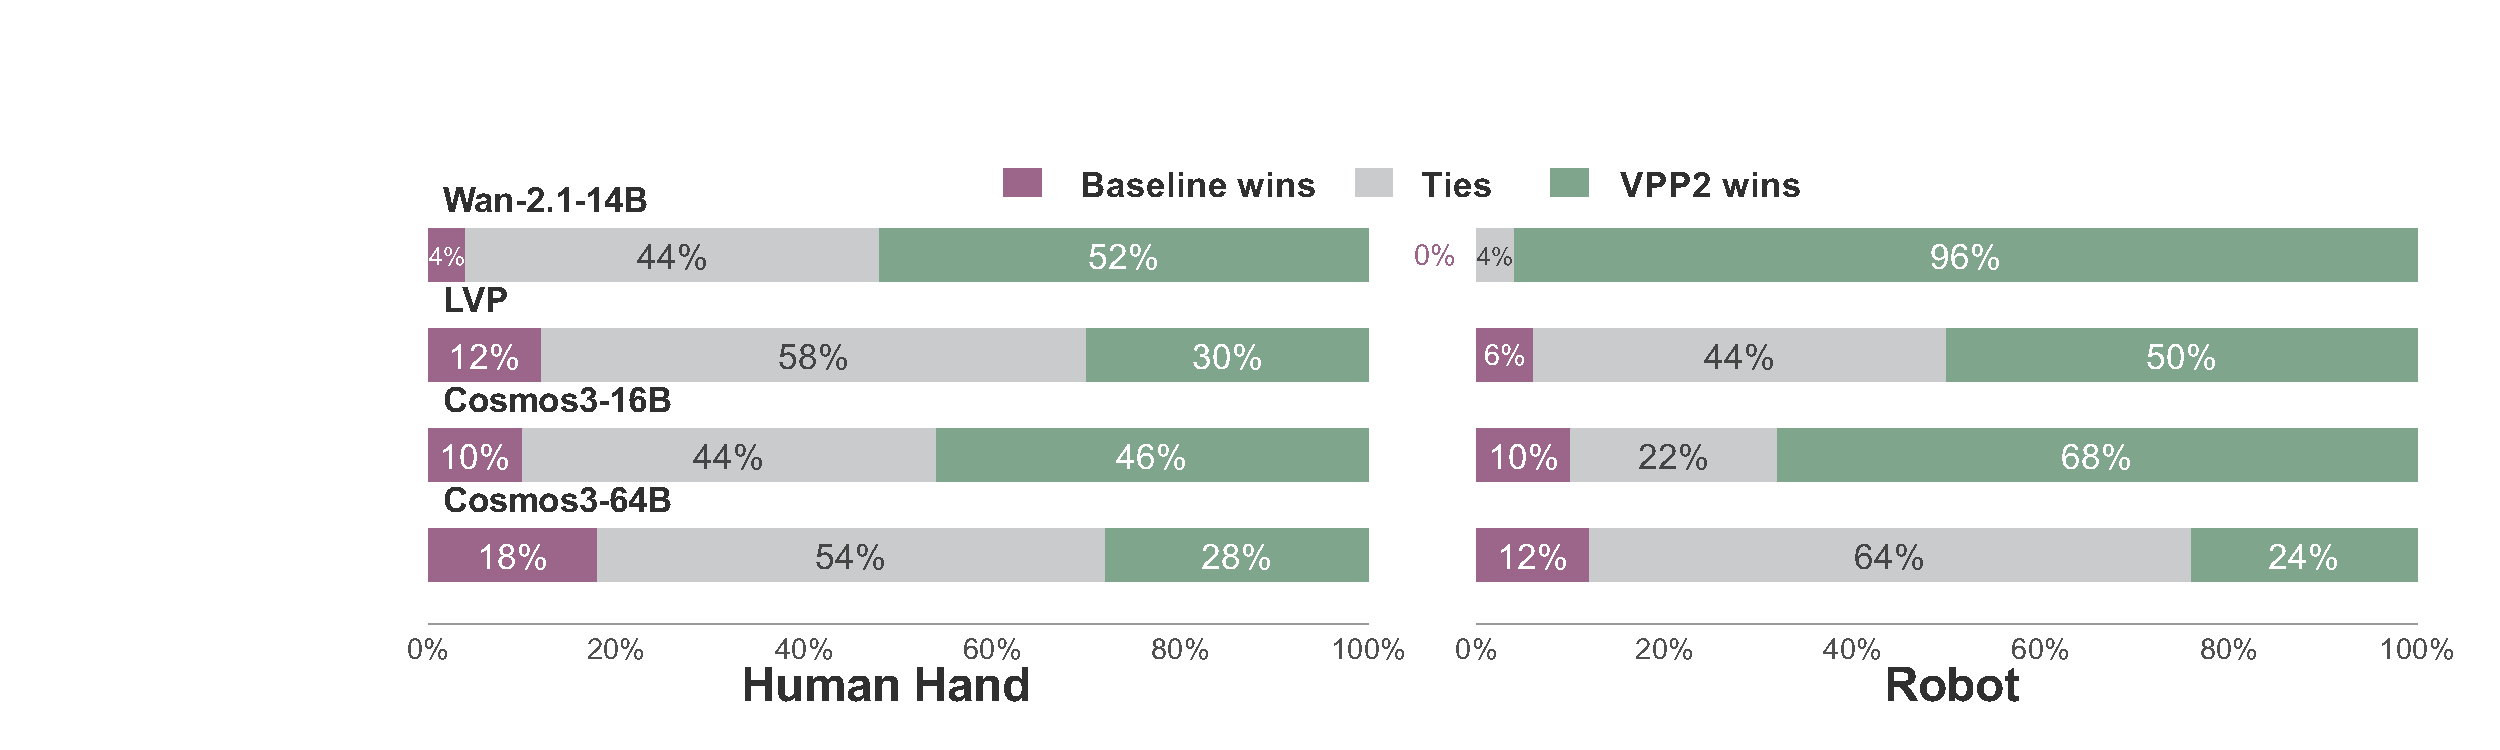
\includegraphics[width=\linewidth]{figures/fig8_2_0921.pdf}

\caption{Win rates of the pretrained VPP2 model against different baselines on video prediction tasks.}
\label{fig:fig8}
\end{minipage}

\end{figure}






\begin{figure}[t]
    \centering
    \vspace{-2mm}
    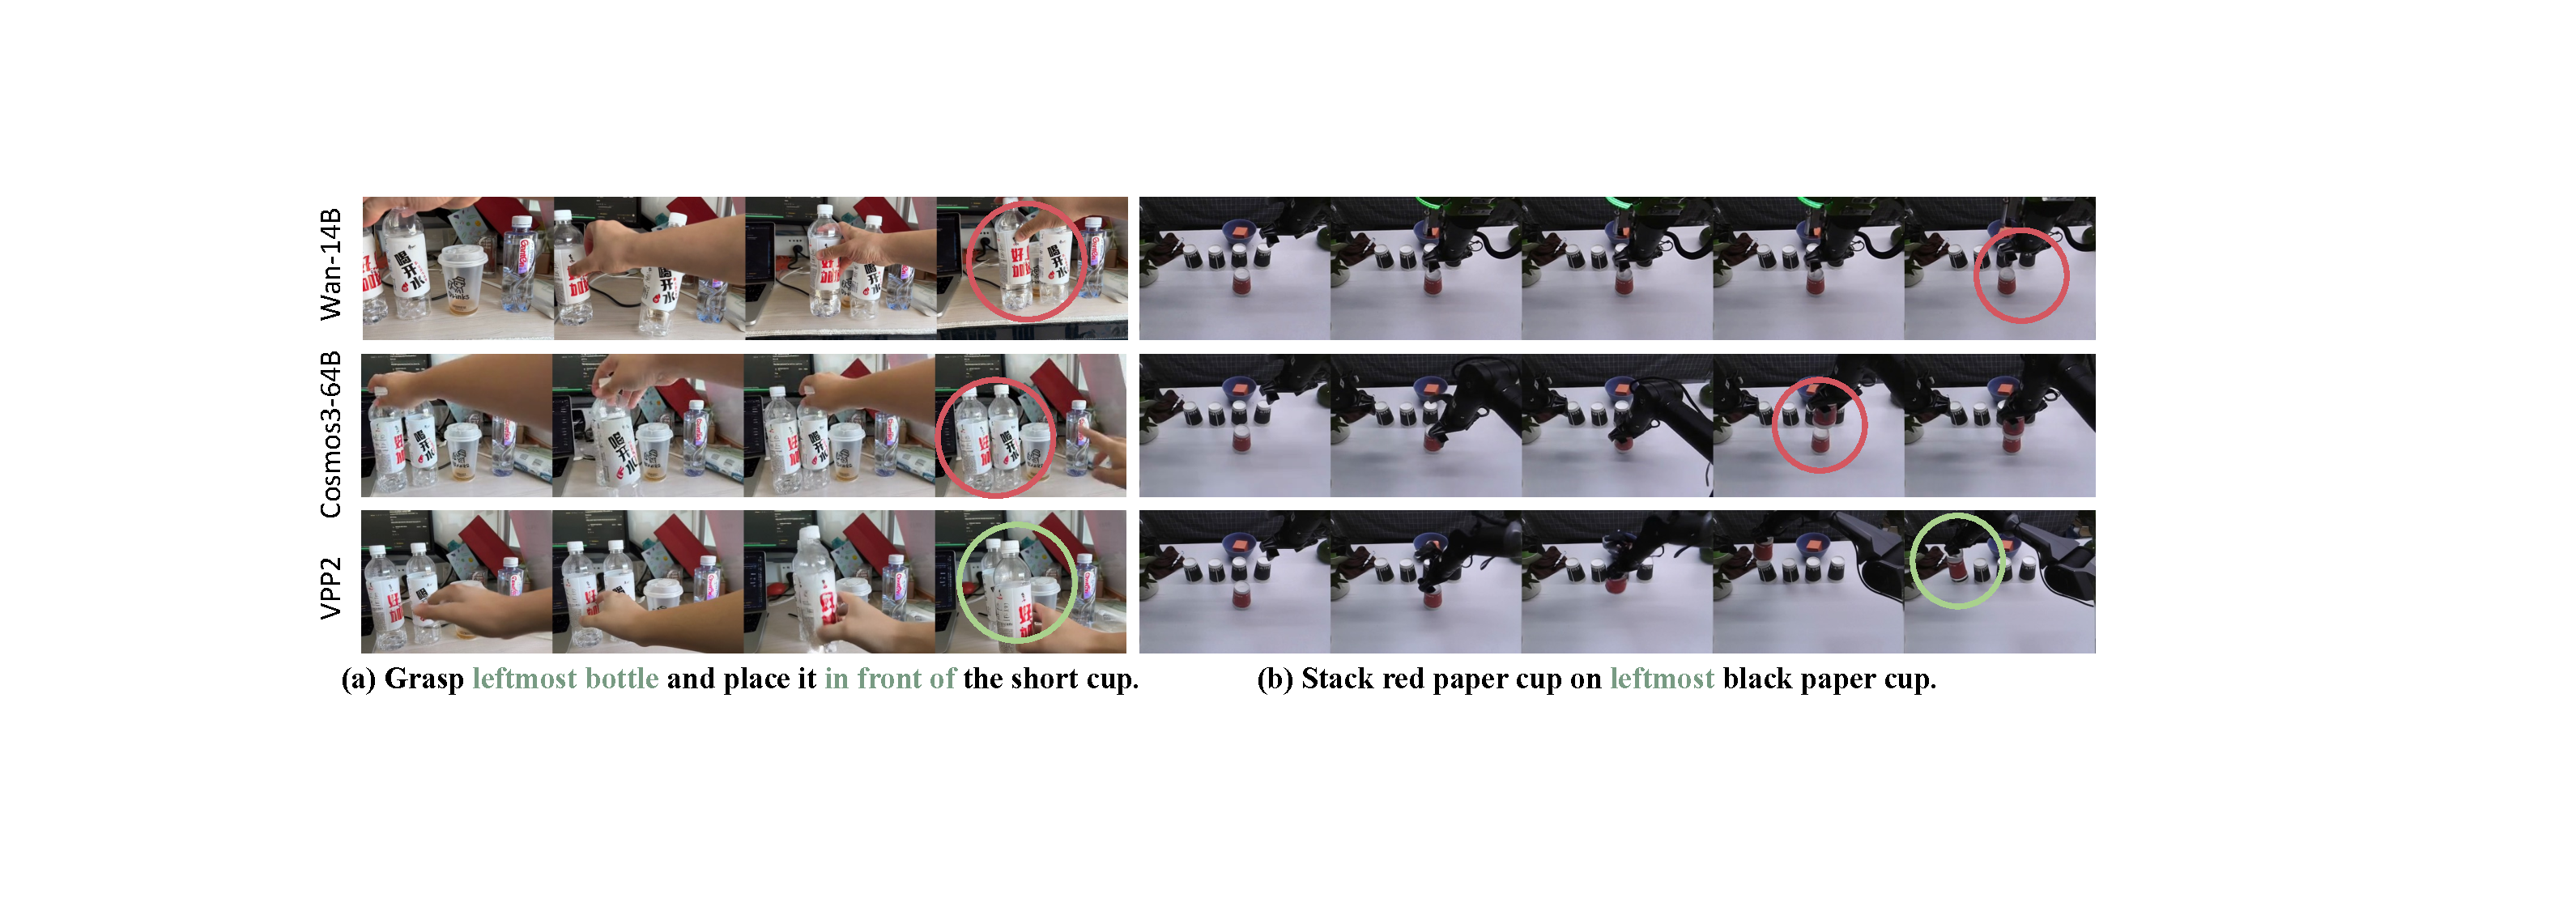
\includegraphics[width=1.0\linewidth]{figures/fig5_2.pdf}
    \caption{Comparison of instruction-following capabilities among VPP2, Wan-14B, and Cosmos3-64B. VPP2 demonstrates better instruction following on complex tasks requiring spatial understanding.}
    \label{fig:fig5}
    \vspace{-4mm}
\end{figure}



% Add to the preamble
% \usepackage{booktabs,tabularx,caption,graphicx}

% Main content




\subsection{Policy Performance Analysis}
\textbf{Zero-shot Performance on Real-world Aloha Robot.} After pretraining a strong video foundation model for manipulation, we post-train and distill it into a fast, single-step generator to support action learning.
With its generalizable video predictions, VPP2 demonstrates strong zero-shot capabilities across open-ended manipulation tasks. We deploy VPP2 directly on a robot embodiment seen during training, without task-specific fine-tuning. For comparison, we train $\pi_{0.5}$~\citep{intelligence2025pi_} and the Wan-14B version of Fast-WAM~\citep{yuan2026fastwam} on the same data used in VPP2 training.
We evaluate models on 10 different categories of zero-shot tasks and present results in Figure~\ref{fig:fig9}. VPP2 achieves an average success rate of 58.5\%, compared with 40.0\% for $\pi_{0.5}$ and 20.5\% for Fast-WAM, and performs best in 9 of the 10 categories.

\begin{figure}[t]
    \centering
    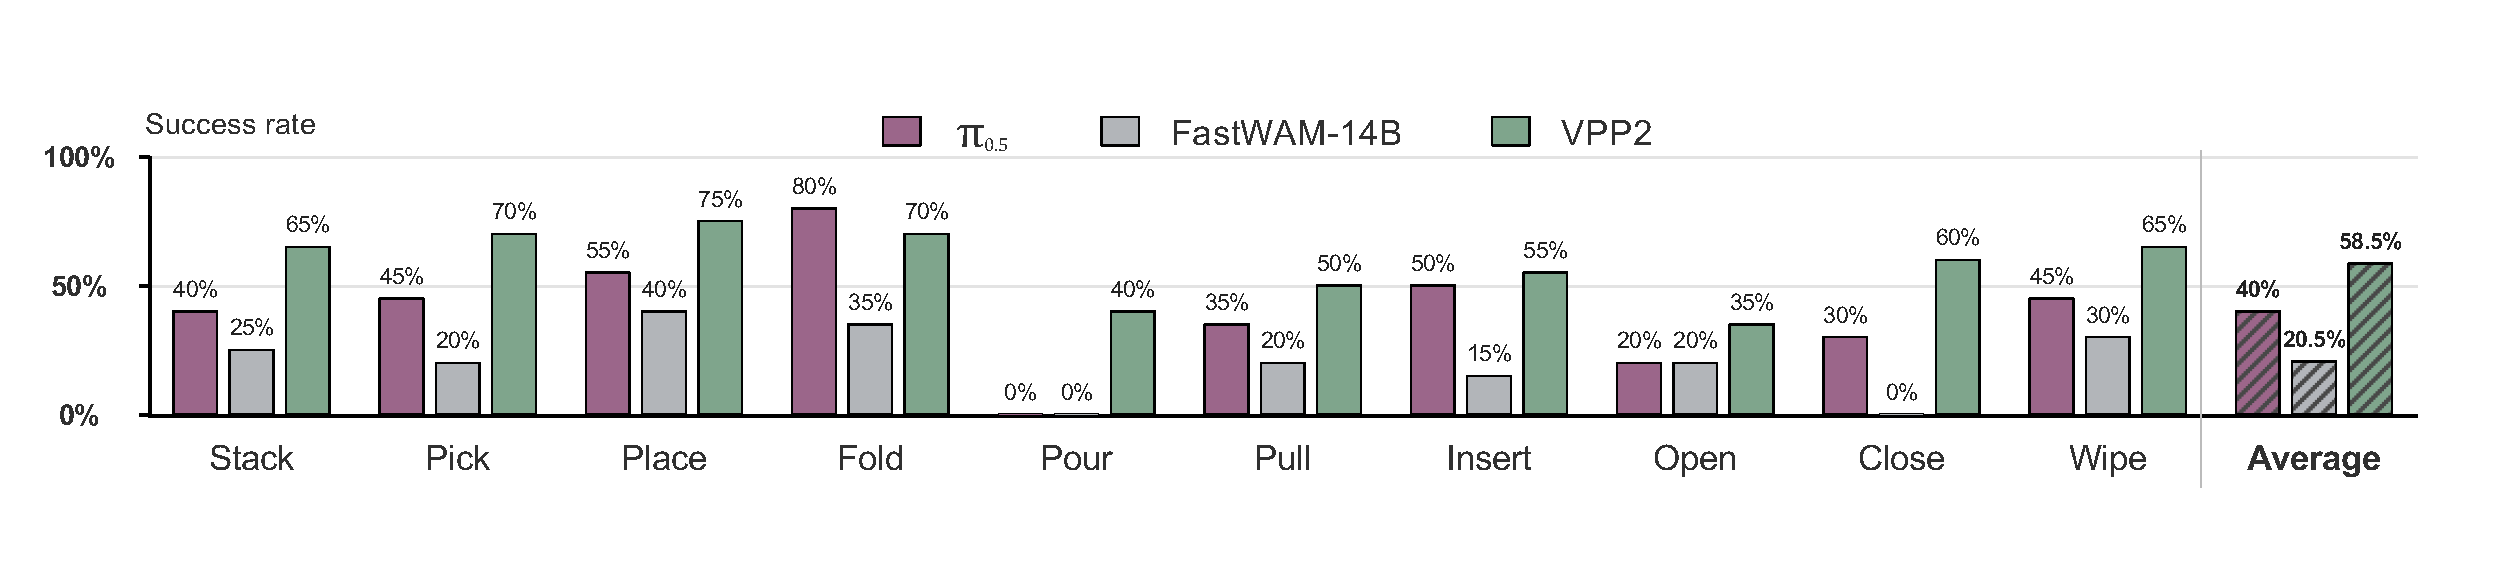
\includegraphics[width=1.0\linewidth]{figures/fig10.pdf}
    \caption{Zero-shot success rates on the real-world ALOHA across 10 randomly selected task categories. For a fair comparison, we finetune $\pi_{0.5}$ and FastWAM on all ALOHA datasets exposed in VPP2’s training data and use the 14B variant of FastWAM.}
    \label{fig:fig9}
    \vspace{-2mm}
\end{figure}


\begin{table*}[t]
\centering

\setlength{\tabcolsep}{5.0pt}
\renewcommand{\arraystretch}{1.0}

\resizebox{0.9\textwidth}{!}{
\begin{tabular}{l c ccc cccc}
\toprule
& \multicolumn{1}{c}{\textbf{LIBERO-ID}}
& \multicolumn{3}{c}{\textbf{LIBERO-Pro}}
& \multicolumn{4}{c}{\textbf{LIBERO-OOD}} \\
\cmidrule(lr){2-2}
\cmidrule(lr){3-5}
\cmidrule(lr){6-9}

\textbf{Method}
& \textbf{Overall}
& \textbf{Position}
& \textbf{Task}
& \textbf{Overall}
& \textbf{Spatial}
& \textbf{Object}
& \textbf{Goal}
& \textbf{Overall} \\
\midrule

$\pi_0$~\citep{black2024pi_0}
& 94.2
& 0.5 & 0.0 & 0.3
& 0.7 & 0.3 & 4.3 & 1.7 \\

$\pi_{0.5}$~\citep{intelligence2025pi_}
& 96.9
& 20.8 & 1.3 & 11.0
& 36.7 & 2.3 & 41.7 & 26.8 \\

MolmoAct~\citep{lee2025molmoact}
& 86.6
& 1.5 & 1.5 & 1.5
& -- & -- & -- & -- \\

X-VLA~\citep{zheng2026xvla}
& 98.1
& 0.8 & 6.8 & 3.8
& -- & -- & -- & -- \\

AtomVLA~\citep{sun2026atomvla}
& 97.0
& 7.3 & 5.3 & 6.3
& -- & -- & -- & -- \\


\midrule

Cosmos-Policy~\citep{kim2026cosmospolicy}
& 98.5
& -- & -- & --
& 30.7 & 0.3 & 0.7 & 10.5 \\

Fast-WAM~\citep{yuan2026fastwam}
& 97.6
& -- & -- & --
& 12.7 & 0.0 & 15.7 & 9.4 \\

DiT4DiT~\citep{ma2026dit4dit}
& 98.6
& -- & -- & --
& 9.0 & 0.0 & 10.3 & 6.4 \\

Temporal Ratio~\citep{mishra2026understanding}
& 94.0
& -- & -- & --
& 58.6 & 40.0 & 80.3 & 59.4 \\

\midrule

\textbf{VPP2 (Ours)}
& \textbf{98.8}
& \textbf{42.3}
& \textbf{47.8}
& \textbf{45.0}
& \textbf{59.3}
& \textbf{44.5}
& \textbf{87.7}
& \textbf{63.9} \\


\bottomrule
\end{tabular}
}
\caption{
Post-training on LIBERO-ID, LIBERO-Pro, and LIBERO-OOD benchmarks.
All models are trained exclusively on the four standard LIBERO suites~\citep{liu2023libero} and are evaluated under three complementary settings.
% For LIBERO-Pro, Position and Task are macro-averaged over the corresponding position and task perturbations across the evaluated suites.
% LIBERO-OOD evaluates compositional generalization along the spatial, object, and goal dimensions.
% Overall denotes the average success rate within each benchmark.
}
\label{tab:libero_generalization}
\vspace{-2mm}
\end{table*}

\begin{table}[t]
\centering
\setlength{\tabcolsep}{4pt}
\resizebox{\textwidth}{!}{
\begin{tabular}{lcccccccc}
\toprule
 & $\pi_0$ & $\pi_{0.5}$ & X-VLA & Fast-WAM & OpenWAM-$\alpha$ & Xiaomi-Robotics-1 & GPT-6-Astra & \textbf{VPP2 (Ours)} \\
\midrule
Avg.\ Score & 3.48 & 11.44 & 10.13 & 3.48 & 17.18 & 20.07 & 28.97 & \textbf{39.26} \\
Success Rate (\%) & 1.53 & 6.93 & 6.52 & 2.03 & 11.92 & 13.93 & 22.48 & \textbf{32.26} \\
\bottomrule
\end{tabular}
}
\caption{Post-training results on the RoboDojo simulation benchmark. Average score captures partial task progress, and success rate measures binary task completion; both are averaged over the five capability dimensions. Baseline results are taken from the official leaderboard.}
\label{tab:robodojo}
\end{table}

\textbf{LIBERO-ID, LIBERO-Pro, and LIBERO-OOD Benchmarks.}
All models are trained exclusively on the four standard LIBERO suites~\citep{liu2023libero} and are evaluated under three complementary settings. LIBERO-ID measures standard in-distribution manipulation performance. To assess generalization beyond the training distribution, we further evaluate on LIBERO-Pro~\citep{zhou2025liberopro} and LIBERO-OOD~\citep{li2025vlas} without additional training. Following HarnessVLA~\citep{zhang2026harness}, we evaluate the Position and Task perturbations of LIBERO-Pro, which test generalization to changes in object positions and task specifications, respectively. We further follow~\citep{mishra2026understanding} to evaluate compositional generalization on LIBERO-OOD, which recombines familiar objects, layouts, and goals into unseen task configurations along spatial, object, and goal dimensions. Per-suite LIBERO-ID results are provided in Appendix~\ref{app_libero}.

As shown in Table~\ref{tab:libero_generalization}, while most baselines exceed 94\% on LIBERO-ID, this in-distribution performance does not transfer to generalization. On LIBERO-Pro, VLA baselines drop to at most 11.0\% overall, whereas VPP2 reaches 45.0\%, with the largest gain on the Task perturbation (47.8\% vs.\ 6.8\%), indicating that VPP2 follows the given instruction rather than replaying memorized trajectories. On LIBERO-OOD, video-based policies such as Cosmos-Policy, Fast-WAM, and DiT4DiT reach at most 10.5\%, while VPP2 achieves 63.9\%, also surpassing Temporal Ratio~\citep{mishra2026understanding}, which specifically targets this generalization gap. We attribute these gains to next-event video prediction with detailed captions, which establishes consistent mappings from instructions to future trajectories.

\textbf{RoboDojo Benchmark.}
RoboDojo~\citep{chen2026robodojo} is a unified sim-and-real benchmark for evaluating generalist robot manipulation policies. Its simulation benchmark contains 42 bimanual tasks covering five capability dimensions: generalization, memory, precision, long-horizon execution, and open-vocabulary instruction following. We follow the official training and evaluation protocol and report both the success rate and the average score, which captures partial task progress.

As shown in Table~\ref{tab:robodojo}, VPP2 achieves an average score of 39.26 and a success rate of 32.26\%, achieving state-of-the-art performance.\footnote{Baseline results are taken from the official RoboDojo simulation leaderboard as of September 2026.} It outperforms representative VLAs such as $\pi_{0.5}$~\citep{intelligence2025pi_}, X-VLA~\citep{zheng2026xvla}, and Xiaomi-Robotics-1~\citep{guo2026xiaomirobotics1}, world action models such as Fast-WAM~\citep{yuan2026fastwam} and OpenWAM-$\alpha$~\citep{wang2026openwam}, and the frontier foundation model GPT-6-Astra~\citep{zhang2026astra} (28.97 / 22.48\%). Per-dimension results are provided in Appendix~\ref{app_robodojo}.



\textbf{VPP2 with Subtask Planning.}
The VPP2 results in Table~\ref{tab:robodojo} use full-task instructions without subtask planning. We further investigate VLM-based subtask planning on five selected RoboDojo task groups covering object classification, block stacking, block swapping, mahjong, and tic-tac-toe. To train the subtask-conditioned policy, we segment demonstrations and pair each segment with a subtask instruction. At test time, a vision-language model (VLM) uses visual observations and execution feedback to select the next subtask for VPP2 to execute.

Figure~\ref{fig:subtask_planning} summarizes the results across the five selected task groups. The evaluated planning configurations achieve an average success rate of 57.6\%, compared with 27.6\% for the baseline. The largest gains occur in language-conditioned block stacking (10\% to 52\%) and tic-tac-toe (0\% to 38\%).

\begin{figure}[t]
    \centering
    \vspace{-3mm}
    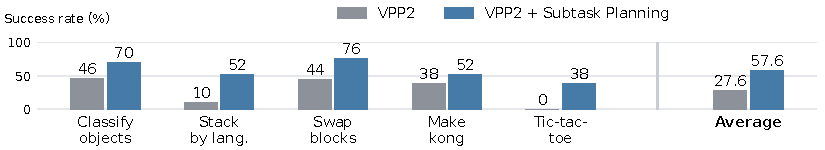
\includegraphics[width=\linewidth]{figures/subtask_planning.pdf}
    \caption{Success rates with and without VLM-based subtask planning (50 trials per task). Average is the five-task mean; the baseline checkpoint matches Table~\ref{tab:robodojo}.}
    \label{fig:subtask_planning}
    \vspace{-3mm}
\end{figure}
